\documentclass{memoir}

\usepackage{amsthm,amssymb,amsmath}
\usepackage{makeidx}
\usepackage{xifthen}
\usepackage[inline]{enumitem}
\usepackage{tikz}
  \usetikzlibrary{patterns}
  \usetikzlibrary{cd}
  \usetikzlibrary{calc}
  \usetikzlibrary{arrows}
\usepackage[framemethod=tikz,usetwoside]{mdframed}
\usepackage{hyperref}
  \hypersetup{linktocpage,colorlinks,linkcolor=blue}
\usepackage[figurewithin=section]{caption}
\usepackage{collect}
\usepackage{wasysym}

%-----------%
% #Counters %
%-----------%

% Number chapters as 0, I, II, III, etc.
\renewcommand{\thechapter}{%
  \ifcase\value{chapter}\relax 0\else \Roman{chapter}\fi%
}%

% Keep chapter numbers and titles from overlapping in TOC
\renewcommand{\chapternumberlinebox}[2]{\makebox[1cm][l]{#2}}

% Number sections sequentially (not within chapters)
\counterwithout{section}{chapter}

% Number figures and tables within sections
\makeatletter                        %&%
  \renewcommand\@memmain@floats{     %&%
    \counterwithout{figure}{chapter} %&%
    \counterwithin{figure}{section}  %&%
    \counterwithout{table}{chapter}  %&%
    \counterwithin{table}{section}   %&%
  }                                  %&%
\makeatother                         %&%




%--------------------------%
% Custom list environments %
%--------------------------%

% See documentation for package enumitem

% Roman-enumerated lists for propositions
\newlist{proplist}{enumerate}{2}
\setlist[proplist]{label=(\roman*)}

% proplist with less vertical space
\newlist{proplist*}{enumerate}{2}
\setlist[proplist*]{label=(\roman*),itemsep=2pt}

% Inline version of proplist
\newlist{inlineproplist}{enumerate}{2}
\setlist[inlineproplist]{label=(\roman*)}


% Arabic-enumerated lists for case analysis
\newlist{caselist}{enumerate}{2}
\setlist[caselist]{align=left,label=\textbf{Case \arabic*:}}
\newcommand{\caseitem}[1]{\item #1}

% Inline version of caselist
\newlist{inlinecaselist}{enumerate}{2}
\setlist[inlinecaselist]{align=left,label=\textbf{Case \arabic*:}}



%------------%
% References %
%------------%

% Subreferences
\newcommand{\sref}[2]{\ref{#1}\ref{#1:#2}}
\newcommand{\paref}[1]{(\ref{#1})}
\newcommand{\eref}[1]{\hyperref[#1]{Exercise \ref*{#1}}}
\newcommand{\propref}[1]{\hyperref[#1]{Proposition \ref*{#1}}}

\def\chapterautorefname{Chapter} %&%
\def\sectionautorefname{Section} %&%
\def\figureautorefname{Figure}   %&%


% Page style
\makepagestyle{standard} %&%

\makeatletter                                                  %&%
\makeevenfoot{standard}{}{}{}                                  %&%
\makeoddfoot{standard}{}{}{}                                   %&%
\makeevenhead{standard}{\bfseries\thepage}{}{\rightmark}       %&%
\makeoddhead{standard}{\leftmark}{}{\bfseries\thepage}         %&%
\makeheadrule{standard}{\textwidth}{\normalrulethickness}      %&%
\makefootrule{standard}{\textwidth}{\normalrulethickness}{0ex} %&%
\makeatother                                                   %&%

\renewcommand*{\sectionmark}[1]{                      %&%
  \markboth{\S\thesection: {#1}}{\S\thesection: {#1}} %&%
}                                                     %&%

\nouppercaseheads    %&%
\pagestyle{standard} %&%
\chapterstyle{dash}  %&%


%----------------%
% Theorem styles %
%----------------%

\theoremstyle{definition}                 %&%
\newtheorem{dfn}{Def'n}[section]          %&%
\newtheorem{thm}[dfn]{Theorem}            %&%
\newtheorem{cor}[dfn]{Cor.}               %&%
\newtheorem{prop}[dfn]{Prop'n}            %&%
\newtheorem{lem}[dfn]{Lemma}              %&%
\newtheorem{construct}[dfn]{Construction} %&%
\newtheorem{axiom}[dfn]{Axiom}            %&%

% Exercises
\newcommand{\Exercises}{\par\bigskip\noindent\hfill{\textasteriskcentered\quad\textasteriskcentered\quad\textsc{\large Exercises}\quad\textasteriskcentered\quad\textasteriskcentered}\hfill\null\par\bigskip}

\newcounter{dummycounter}         %&%
\newcounter{exercise}[section]    %&%
\counterwithin{exercise}{section} %&%

\marginparmargin{left} %&%

\newenvironment{exercise}[1][\unskip]{                     %&%
  \refstepcounter{exercise}                                %&%
  \par\noindent\marginpar{\hfill\theexercise .}\textbf{#1} %&%
}{                                                         %&%
  \medskip                                                 %&%
}                                                          %&%



% Examples
\newenvironment{examples}{                      %&%
  \par\bigskip\noindent\textbf{\large Examples} %&%
  \begin{enumerate}                             %&%
}{                                              %&%
  \end{enumerate}                               %&%
}                                               %&%


\mdfdefinestyle{mystyle}{ %&%
  hidealllines=true,      %&%
  leftline=true,          %&%
  innerleftmargin=10pt,   %&%
  innerrightmargin=10pt,  %&%
  innertopmargin=0pt,     %&%
}                         %&%

\surroundwithmdframed[style=mystyle]{dfn}   %&%
\surroundwithmdframed[style=mystyle]{prop}  %&%
\surroundwithmdframed[style=mystyle]{cor}   %&%
\surroundwithmdframed[style=mystyle]{axiom} %&%



% For nebulous "problem" statements
\newenvironment{titlebox}[1]                       %&%
  {\mdfsetup{                                      %&%
    frametitle={\colorbox{white}{\space#1\space}}, %&%
    innertopmargin=7pt,                            %&%
    innerbottommargin=10pt,                        %&%
    frametitleaboveskip=-\ht\strutbox,             %&%
    frametitlealignment=\center                    %&%
    }                                              %&%
  \begin{mdframed}                                 %&%
  }                                                %&%
  {\end{mdframed}                                  %&%
}                                                  %&%


%---------%
% Numbers %
%---------%

\newcommand{\ZZ}{\ensuremath{\mathbb{Z}}} %&%
\newcommand{\NN}{\ensuremath{\mathbb{N}}} %&%
\newcommand{\QQ}{\ensuremath{\mathbb{Q}}} %&%
\newcommand{\RR}{\ensuremath{\mathbb{R}}} %&%
\newcommand{\CC}{\ensuremath{\mathbb{C}}} %&%

\newcommand{\ZZINT}[2]{\ensuremath{[\![#1,#2]\!]}} %&%



%-----------------------%
% Maps and sets of maps %
%-----------------------%

\newcommand{\ID}[1][]{\ensuremath{ %&%
  \ifthenelse{\isempty{#1}}        %&%
    {\mathsf{id}}                  %&%
    {\mathsf{id}_{#1}}             %&%
}}                                 %&%

\newcommand{\END}[1]{\ensuremath{ %&%
  \mathsf{End}\left(#1\right)     %&%
}}                                %&%

\newcommand{\ENDU}[1]{\ensuremath{ %&%
  \mathsf{End}_1\left(#1\right)    %&%
}}                                 %&%



%--------------%
% Ring subsets %
%--------------%

\newcommand{\CENTER}[1]{\ensuremath{ %&%
  Z\left(#1\right)                   %&%
}}                                   %&%

\newcommand{\NILRADICAL}[1]{\ensuremath{ %&%
  N\left(#1\right)                       %&%
}}                                       %&%

\newcommand{\UNITS}[1]{\ensuremath{ %&%
  \mathcal{U}\left(#1\right)        %&%
}}                                  %&%

\newcommand{\KER}[1]{\ensuremath{ %&%
  \mathsf{ker}(#1)                %&%
}}                                %&%

\newcommand{\IM}[1]{\ensuremath{ %&%
  \mathsf{im}(#1)                %&%
}}                               %&%



%--------------------------%
% Families of ring subsets %
%--------------------------%

\newcommand{\ASSOCLAT}[1]{\ensuremath{ %&%
  \mathcal{A}\left(#1\right)           %&%
}}                                     %&%

\newcommand{\IDEALS}[2][]{\ensuremath{ %&%
  \ifthenelse{\isempty{#1}}            %&%
    {\mathcal{Q}\left(#2\right)}       %&%
    {\mathcal{Q}_{#1}\left(#2\right)}  %&%
}}                                     %&%



%----------%
% Geometry %
%----------%

\newcommand{\COLLINEAR}[3]{\ensuremath{\langle #1, #2, #3 \rangle}}%&%
\newcommand{\LINE}[2]{\ensuremath{\overleftrightarrow{#1#2}}}%&%
\newcommand{\BETWEEN}[3]{\ensuremath{[ #1 #2 #3 ]}}%&%
\newcommand{\SEGMENT}[2]{\ensuremath{\overline{#1#2}}}%&%
\newcommand{\RAY}[2]{\ensuremath{\overrightarrow{#1#2}}}%&%
\newcommand{\TRIANGLE}[3]{\ensuremath{\bigtriangleup{#1#2#3}}}%&%
\newcommand{\ANGLE}[3]{\ensuremath{\angle{#1#2#3}}}%&%
\newcommand{\INTANGLE}[3]{\ensuremath{\mathsf{int}\angle{#1#2#3}}}%&%
\newcommand{\SEGCONG}[4]{\ensuremath{(#1,#2) \cong_s (#3,#4)}}%&%
\newcommand{\ANGCONG}[6]{\ensuremath{(#1,#2,#3) \cong_a (#4,#5,#6)}}%&%
\renewcommand{\CIRCLE}[2]{\ensuremath{\ocircle{#1#2}}}%&%
\newcommand{\INTCIRCLE}[2]{\ensuremath{\mathsf{int}\CIRCLE{#1}{#2}}}
\newcommand{\EXTCIRCLE}[2]{\ensuremath{\mathsf{ext}\CIRCLE{#1}{#2}}}

\newcommand{\HALFPLANEA}[1]{\mathcal{H}_{1,\ell}}
\newcommand{\HALFPLANEB}[1]{\mathcal{H}_{2,\ell}}

\newcommand{\SEPARATE}[4]{\ensuremath{(#1,#2 \mid #3,#4)}}

\newcommand{\HYPHP}{\ensuremath{\mathbb{H}}}
\newcommand{\HHPIDEALPOINT}[2]{\ensuremath{H_{#1,#2}}}

\newcommand{\POINCAREDISC}{\ensuremath{\mathbb{P}}}
\newcommand{\PDDET}[2]{D_{#1,#2}}
\newcommand{\PDIDEALPOINT}[2]{P_{#1,#2}}

\newcommand{\KLEINDISC}{\ensuremath{\mathbb{K}}}
\newcommand{\KDIDEALPOINT}[2]{\ensuremath{K_{#1,#2}}}

\newcommand{\EUCLIDEANDISC}{\ensuremath{\mathbb{E}}}

\newcommand{\ANTIPODALSPHERE}{\ensuremath{\mathbb{A}}}

\newcommand{\MIN}{\ensuremath{\mathsf{min}}}
\newcommand{\MAX}{\ensuremath{\mathsf{max}}}



\newcommand{\TOT}[1]{\ensuremath{\mathsf{tot}\left(#1\right)}}%&%

\newcommand{\POW}[1]{\ensuremath{\mathcal{P}\left(#1\right)}}%&%
\newcommand{\POWP}[1]{\ensuremath{\mathcal{P}_{\!\neq\!}\left(#1\right)}}%&%
\newcommand{\POWF}[1]{\ensuremath{\mathcal{P}_F\left(#1\right)}}%&%

\newcommand{\ZZQUAD}[1]{\ensuremath{\mathcal{O}(\sqrt{#1})}}%&%
\newcommand{\ZZFRAC}[1]{\ensuremath{{#1}^{-1}\ZZ}}%&%

\newcommand{\ION}[1]{\ensuremath{\mathsf{nilp}\left(#1\right)}}%&%

\newcommand{\REXTEND}[3]{\ensuremath{#1 \rtimes_{#2} #3}}%&%
\newcommand{\ADJUNIT}[1]{\ensuremath{{#1}^{(1)}}}%&%
\newcommand{\HAM}[1]{\ensuremath{\mathbb{H}(#1)}}%&%

\newcommand{\ADDORD}[1]{\ensuremath{\mathsf{ord}\left(#1\right)}}%&%
\newcommand{\CHAR}[1]{\ensuremath{\mathsf{char}(#1)}}%&%

\newcommand{\MAT}[2]{\ensuremath{\mathsf{Mat}_{#1}(#2)}}%&%
\newcommand{\UTMAT}[2]{\ensuremath{\mathsf{UT}_{#1}(#2)}}%&%
\newcommand{\LTMAT}[2]{\ensuremath{\mathsf{LT}_{#1}(#2)}}%&%
\newcommand{\DIAGMAT}[2]{\ensuremath{\mathsf{Diag}_{#1}(#2)}}%&%
\newcommand{\DET}{\ensuremath{\mathsf{det}}}%&%

\newcommand{\GCD}[2]{\ensuremath{\mathsf{gcd}(#1, #2)}}%&%
\newcommand{\LCM}[2]{\ensuremath{\mathsf{lcm}(#1, #2)}}%&%
\newcommand{\GCDS}[1]{\ensuremath{\mathsf{gcd}\left(#1\right)}}%&%

\newcommand{\CONTENT}[1]{\ensuremath{\mathsf{content}(#1)}}%&%

\newcommand{\ASSOC}{\ensuremath{\approx}}%&%
\newcommand{\COPRIME}{\ensuremath{\perp}}%&%

\newcommand{\DIVORD}[2]{\ensuremath{\mathsf{div}_{#1}\left(#2\right)}}%&%

\newcommand{\LOCALIZE}[2]{\ensuremath{{#2}^{-1}{#1}}}%&%

\newcommand{\POLYEVAL}[1]{\ensuremath{\varepsilon_{#1}}}%&%
\newcommand{\DERIV}[1][]{\ensuremath{\ifthenelse{\isempty{#1}}{\mathsf{D}}{\mathsf{D}_{#1}}}}%&%

\newcommand{\TILDE}[1]{\ensuremath{\widetilde{#1}}}%&%

\newcommand{\LIM}[2][]{\ensuremath{\ifthenelse{\isempty{#1}}{\lim}{\lim_{#1}}\left(#2\right)}}%&%

\newcommand{\VALCOMP}[2]{\ensuremath{\overline{#1}_{#2}}}%&%


\makeindex

\begin{document}

\title{Elementary Geometrese}
\author{nathan bloomfield}


\frontmatter

\thispagestyle{empty}

\begin{center}
{\Large Elementary Geometrese}

\vspace{1cm}

Nathan Bloomfield

\vspace{3cm}

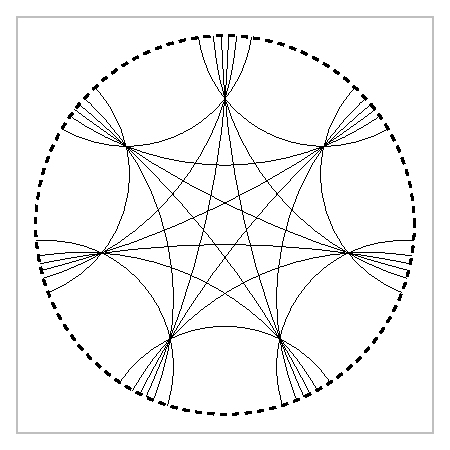
\includegraphics[scale=1.8,trim=4 4 4 4,clip]{src/geo/gfx/cover/cover.eps}
\end{center}

\newpage
\tableofcontents

\setcounter{page}{0}

\begin{center}
\begin{minipage}{0.8\textwidth}
\begin{center}
\vspace{40pt}

This work is licensed under a Creative Commons Attribution NonCommercial ShareAlike 4.0 International License.

\vspace{12pt}

\includegraphics[scale=0.8]{src/geo/gfx/by-nc-sa.eps}
\end{center}
\end{minipage}
\end{center}
\newpage


\mainmatter

\chapter{Incidence}
\newpage

  \section{Models and Theories}
    \input{src/geo/1.01-models-and-theories.tex}
    \newpage

  \section{Incidence Geometry}
    Traditional plane geometry involves many different concepts, including \emph{lines}, \emph{angles}, \emph{congruent}, and many others.
In order to manage the complexity this entails, we will build up our geometries one piece at a time starting here with the idea of \emph{collinearity}.

\begin{dfn}[Incidence Geometry] \label{dfn:incidence-geometry}
Let \(P\) be a set, whose elements we call \emph{points}.
A ternary relation \(\COLLINEAR{\ast}{\ast}{\ast}\) on \(P\) is called a \emph{collinearity relation}\index{collinearity} if the following properties are satisfied.
\begin{proplist}
\item[IG1.] If \(a\), \(b\), and \(c\) are points such that \(\COLLINEAR{a}{b}{c}\), then \(\COLLINEAR{b}{a}{c}\) and \(\COLLINEAR{a}{c}{b}\).
\item[IG2.] If \(a\) and \(b\) are points such that \(a \neq b\), then \(\COLLINEAR{a}{b}{b}\).
\item[IG3.] \(\COLLINEAR{a}{a}{a}\) does not hold for any point \(a\).
\item[IG4.] There exist distinct points \(a\), \(b\), and \(c\) such that \(\COLLINEAR{a}{b}{c}\) does not hold.
\item[IG5.] If \(a\), \(b\), \(u\), and \(v\) are points such that \(a \neq b\), \(u \neq v\), \(\COLLINEAR{a}{b}{u}\), and \(\COLLINEAR{a}{b}{v}\), then \(\COLLINEAR{a}{u}{v}\).
\end{proplist}
If such a relation exists we say that \((P, \COLLINEAR{\ast}{\ast}{\ast})\) is an \emph{incidence geometry}\index{incidence geometry}.
In this case, when \(\COLLINEAR{a}{b}{c}\) we say that \(a\), \(b\), and \(c\) are \emph{collinear}.
\end{dfn}

It is important to remember that the word ``collinear'' here is an undefined term, and we have to try very hard not to think of ordinary lines and points when using it.
(This is part of the theory-model confusion we inherit from history.)
The meaning of the word ``collinear'' is determined precisely by how it is used in the incidence geometry axioms, and only becomes concrete when we specify a particular model.
In particular, it does not make sense to draw pictures of the points in an arbitrary incidence geometry!

Although ``collinear'' is an abstract, undefined term, we'd like for it to behave much like our intuition expects.
We want this undefined term to \emph{formalize} our intuition about collinearity.
To that end, note that collinearity satisfies some additional basic properties.

\begin{prop}
Let \(P\) be an incidence geometry.
Then we have the following for all points \(a\), \(b\), and \(c\).
\begin{proplist}
\item If \(\COLLINEAR{a}{b}{c}\), then we also have \(\COLLINEAR{b}{c}{a}\), \(\COLLINEAR{c}{a}{b}\), and \(\COLLINEAR{c}{b}{a}\).
\item If \(a \neq b\), then \(\COLLINEAR{a}{b}{a}\) and \(\COLLINEAR{b}{a}{a}\).
\end{proplist}
\end{prop}

It may seem strange to define ``collinear'' before we define ``line''; typically we think of points being collinear precisely when there is a unique line containing all of them.
But we can just as easily define lines in terms of collinearity as follows.

\begin{dfn}[Line] \label{dfn:line}
Let \(P\) be an incidence geometry with distinct points \(a\) and \(b\).
We define the \emph{line}\index{line} through \(a\) and \(b\) to be the set \[ \LINE{a}{b} = \{ c \in P \mid \COLLINEAR{a}{b}{c} \}. \]
If \(c \in \LINE{a}{b}\), we say that \(c\) \emph{lies on} \(\LINE{a}{b}\).
\end{dfn}

That is, the line through \(a\) and \(b\) is precisely the set of points which are collinear with \(a\) and \(b\).
Remember: it is vital that we not think about drawings of points and lines here.
In an arbitrary incidence geometry, ``point'' and ``line'' are just \emph{words} which we assume have a particular relationship with one another.
Thinking at this level of abstraction may seem unnecessarily difficult at first, but -- and it is difficult to overstate this -- the abstract way of thinking brings enormous power.
Here are some basic properties of lines which can be derived from the properties of collinearity alone.

\begin{prop}
Let \(P\) be an incidence geometry.
Then the following hold for all distinct points \(a\) and \(b\) in \(P\).
\begin{proplist}
\item \(a \in \LINE{a}{b}\) and \(b \in \LINE{a}{b}\).
\item \(\LINE{a}{b} = \LINE{b}{a}\).
\item If \(c \in \LINE{a}{b}\) and \(c \neq a\), then \(\LINE{a}{c} = \LINE{a}{b}\).
\item If \(u,v \in \LINE{a}{b}\) are distinct points, then \(a,b \in \LINE{u}{v}\).
\end{proplist}
\end{prop}

Though we will eventually have several examples of incidence geometry, it is crucial when proving theorems that we not rely on any specific model.
This is the power of abstraction: any theorem which depends only on properties common to \emph{all} incidence geometries immediately holds in \emph{any} incidence geometry.
For example, consider the following theorem.

\begin{prop}[Line Intersection]
Let \(P\) be an incidence geometry with lines \(\ell_1\) and \(\ell_2\).
Then exactly one of the following holds.
\begin{proplist}
\item \(\ell_1 = \ell_2\), and we say \(\ell_1\) and \(\ell_2\) are \emph{coincident}\index{coincident lines},
\item \(\ell_1 \cap \ell_2 = \varnothing\), and we say \(\ell_1\) and \(\ell_2\) are \emph{disjoint}\index{disjoint lines}, or
\item \(\ell_1 \cap \ell_2 = \{p\}\) for some point \(p\), and we say \(\ell_1\) and \(\ell_2\) are \emph{incident}\index{incident lines}.
\end{proplist}
In the first two cases (coincident or disjoint) we say that \(\ell_1\) and \(\ell_2\) are \emph{parallel}\index{parallel lines}.
\end{prop}

\begin{proof}
Suppose \(\ell_1 \cap \ell_2\) contains at least two points, say \(x\) and \(y\).
Then in fact \(\ell_1 = \LINE{x}{y} = \ell_2\).
So if \(\ell_1 \neq \ell_2\) then \(\ell_1 \cap \ell_2\) contains either exactly one or zero points.
\end{proof}

This theorem holds in any model of incidence geometry.
One problem: we don't have any models of incidence geometry yet!
We'll fix this in the next section.



%---------%
\Exercises%
%---------%

\begin{exercise}\label{exerc:rr2-collinear-comb}
Let \(A = (a_x, a_y)\), \(B = (b_x, b_y)\), and \(C = (c_x, c_y)\) be in \(\RR^2\) such that \(A \neq B\).
Show that \[ \DET \begin{bmatrix} a_x & a_y & 1 \\ b_x & b_y & 1 \\ c_x & c_y & 1 \end{bmatrix} = 0 \] if and only if \(C = A + t(B - A)\) for some unique \(t \in \RR\).
(Hint: Consider \[ \frac{c_x - a_x}{b_x - a_x} = \frac{c_y - a_y}{b_y - a_y} \].)
\end{exercise}

\begin{dfn}[Collineation]
Suppose we have incidence geometries \(P\) and \(Q\).
A bijective mapping \(\varphi : P \rightarrow Q\) is called a \emph{collineation}\index{collineation} if, for all points \(x,y,z \in P\), whenever \(\COLLINEAR{x}{y}{z}\) in \(P\), we also have \(\COLLINEAR{\varphi(x)}{\varphi(y)}{\varphi(z)}\) in \(Q\).
\end{dfn}

\begin{exercise}
Prove the following.
\begin{proplist}
\item If \(P\) is an incidence geometry, then the identity map \(1 : P \rightarrow P\) is a collineation.
\item If \(\varphi : P \rightarrow Q\) and \(\psi : Q \rightarrow R\) are collineations, then \(\psi \circ \varphi\) is a collineation.
\item If \(\varphi : P \rightarrow Q\) is a collineation, then \(\varphi^{-1} : Q \rightarrow P\) is a collineation.
\end{proplist}
\end{exercise}

    \newpage

  \section{Parallel Lines}
    \input{src/geo/1.03-parallel-lines.tex}
    \newpage

  \section{Collineations}
    Collinearity relations represent a kind of \emph{abstract structure}.
Typically in mathematics, whenever we have a kind of structure, the mappings which \emph{preserve} that structure are interesting.
In the case of an incidence geometry such mappings are called \emph{collineations}.

\begin{dfn}[Collineation]
Suppose we have incidence geometries \(P\) and \(Q\).
A bijective mapping \(\varphi : P \rightarrow Q\) is called a \emph{collineation}\index{collineation} if, for all points \(x,y,z \in P\), whenever \(\COLLINEAR{x}{y}{z}\) in \(P\), we also have \(\COLLINEAR{\varphi(x)}{\varphi(y)}{\varphi(z)}\) in \(Q\).
\end{dfn}

\begin{prop}
We have the following.
\begin{proplist}
\item If \(P\) is an incidence geometry, then the identity map \(1 : P \rightarrow P\) is a collineation.
\item If \(\varphi : P \rightarrow Q\) and \(\psi : Q \rightarrow R\) are collineations, then \(\psi \circ \varphi\) is a collineation.
\item If \(\varphi : P \rightarrow Q\) is a collineation, then \(\varphi^{-1} : Q \rightarrow P\) is a collineation.
\end{proplist}
\end{prop}



%---------%
\Exercises%
%---------%

\begin{exercise}
Let \(\varphi : \RR^2 \rightarrow \RR^2\) be given by \[ \varphi(X) = MX + B, \]
where \(M\) is an invertible \(2 \times 2\) matrix over \(\RR\) and \(B \in \RR^2\).
Show that \(\varphi\) is a collineation.
\end{exercise}



\chapter{Order}
\newpage

  \section{Betweenness}
    \input{src/geo/2.01-betweenness.tex}
    \newpage

  \section{Ordered Geometry}
    The existence of a betweenness relation on an incidence geometry says something very strong.
Combined with an additional property -- the Line Separation property -- such geometries are called \emph{ordered}.

\begin{dfn}[Ordered Geometry]
Let \(P\) be an incidence geometry with a betweenness relation \(\BETWEEN{\ast}{\ast}{\ast}\).
We say that \(P\) is an \emph{ordered geometry} if it satisfies the following additional \emph{Line Separation Property}.
\begin{itemize}
\item[LS.] For every line \(\ell\) there are two sets, \(\HALFPLANEA{\ell}\) and \(\HALFPLANEB{\ell}\), which satisfy the following properties.
\begin{proplist}
\item \(\HALFPLANEA{\ell}\) and \(\HALFPLANEB{\ell}\) are not empty.
\item \(\ell\), \(\HALFPLANEA{\ell}\), and \(\HALFPLANEB{\ell}\) partition \(P\).
\item \(\HALFPLANEA{\ell}\) and \(\HALFPLANEB{\ell}\) are convex.
\item If \(x \in \HALFPLANEA{\ell}\) and \(y \in \HALFPLANEB{\ell}\), then \(\SEGMENT{x}{y} \cap \ell = \{p\}\) for some point \(p\).
\end{proplist}
The sets \(\HALFPLANEA{\ell}\) and \(\HALFPLANEB{\ell}\) are called \emph{halfplanes}\index{halfplane}.
\end{itemize}
\end{dfn}

The Line Separation property essentially states that every line divides the plane into two ``separate'' pieces -- we might call these pieces the \emph{sides} of the line.
Given a line \(\ell\) and points \(x,y \notin \ell\), we say that \(x\) and \(y\) are on the \emph{same side} of \(\ell\) if they are both in the same halfplane bounded by \(\ell\), and otherwise they are on \emph{opposite sides}.
See \autoref{fig:line-sep} for a picture.
(But remember that a given ordered geometry might look very different!)

\begin{figure}[h]
\begin{center}
\begin{tikzpicture}
  \draw [<->] (0,0) -- (2,4);
  \coordinate [label=below right:\(\ell\)] (x) at (1,2);
  \node at (-1,2) {\(\HALFPLANEA{\ell}\)};
  \node at (2.5,2) {\(\HALFPLANEB{\ell}\)};
\end{tikzpicture}
\caption{\label{fig:line-sep}The halfplanes bounded by a line.}
\end{center}
\end{figure}

\begin{dfn}[Triangle]
Let \(P\) be an incidence geometry, and let \(x\), \(y\), and \(z\) be points.
Then the set \[ \TRIANGLE{x}{y}{z} = \SEGMENT{x}{y} \cup \SEGMENT{y}{z} \cup \SEGMENT{z}{x} \] is called the \emph{triangle} with \emph{vertices} \(x\), \(y\), and \(z\).
The segments \(\SEGMENT{x}{y}\), \(\SEGMENT{y}{z}\), and \(\SEGMENT{z}{x}\) are called the \emph{sides}\index{sides (of a triangle)} of the triangle, and the lines \(\LINE{x}{y}\), \(\LINE{y}{z}\), and \(\LINE{z}{x}\) are called the \emph{extended sides}\index{extended sides (of a triangle)}.
If \(x\), \(y\), and \(z\) are not all distinct, we say that the triangle \(\TRIANGLE{x}{y}{z}\) is \emph{degenerate}\index{degenerate!triangle}.
\end{dfn}

The next result seems intuitive, but must be proven; it states that if a line ``enters'' a triangle through one side and does not contain any of the triangle's vertices, then it must ``exit'' the triangle through one of the other sides.
This is called \emph{Pasch's Axiom} for historical reasons.

\begin{prop}[Pasch's Axiom]
Let \(x\), \(y\), and \(z\) be distinct noncollinear points in an ordered geometry, and let \(\ell\) be a line such that \(x,y,z \notin \ell\).
Finally, suppose there is a point \(w \in \ell\) such that \(\BETWEEN{x}{w}{y}\); that is, \(\ell\) cuts the side \(\SEGMENT{x}{y}\).
Then precisely one of the following two things happens:
\begin{proplist}
\item \(\ell\) cuts \(\SEGMENT{y}{z}\) and does not cut \(\SEGMENT{z}{x}\), or
\item \(\ell\) cuts \(\SEGMENT{z}{x}\) and does not cut \(\SEGMENT{y}{z}\).
\end{proplist}
\end{prop}

\begin{proof}
Since \(P\) is an ordered geometry, it satisfies the Plane Separation property.
In particular, the points not on \(\ell\) are partitioned into two convex, nonempty half-planes, \(\HALFPLANEA{\ell}\) and \(\HALFPLANEB{\ell}\).
Since \(x\) and \(y\) are not on \(\ell\), without loss of generality we have \(x \in \HALFPLANEA{\ell}\) and \(y \in \HALFPLANEB{\ell}\).
Since \(z \notin \ell\), there are two possibilities: either \(z \in \HALFPLANEA{\ell}\) or \(z \in \HALFPLANEB{\ell}\).
In the first case, we see that \(\ell\) cuts \(\SEGMENT{y}{z}\) and does not cut \(\SEGMENT{z}{x}\), and in the second case, \(\ell\) cuts \(\SEGMENT{z}{x}\) but not \(\SEGMENT{y}{z}\).
\end{proof}

In other words, Pasch's Axiom states that if a line enters a triangle then it must also exit; see Figure \ref{fig:pasch}.

\begin{figure}[h]
\begin{center}
\begin{tikzpicture}[scale=1.1]
  \coordinate [label=below:\(x\)] (X) at (0,0);
  \coordinate [label=above left:\(y\)] (Y) at (-1,2);
  \coordinate [label=right:\(z\)] (Z) at (4,1);
  \coordinate (H) at (0,1);
  \coordinate (K) at (-2,2);
  \draw (X) -- (Y) -- (Z) -- cycle;
  \draw [->] (H) -- (K);
  \coordinate [label=below left:\(w\)] (W) at (intersection of X--Y and H--K);
  \draw [->,dashed] (H) -- (1,0.5);
  \draw [fill] (X) circle [radius=0.7pt];
  \draw [fill] (Y) circle [radius=0.7pt];
  \draw [fill] (Z) circle [radius=0.7pt];
  \draw [fill] (W) circle [radius=0.7pt];
\end{tikzpicture}
\caption{\label{fig:pasch}The setup of Pasch's Axiom}
\end{center}
\end{figure}

\begin{lem}\label{lem:betweenness-separation}
Let \(\ell\) be a line and \(C \in \ell\) a point in an ordered geometry.
Suppose \(A\) and \(B\) are points not on \(\ell\) such that \(\BETWEEN{A}{B}{C}\).
Then \(A\) and \(B\) are on the same side of \(\ell\).
\end{lem}

\begin{proof}
Suppose otherwise that \(A\) and \(B\) are on opposite sides of \(\ell\).
By the Line Separation property, and because \(A\) and \(B\) are not on \(\ell\), the segment \(\SEGMENT{A}{B}\) cuts \(\ell\) at a unique point \(D\).
That is, \(D \in \ell\) and \(\BETWEEN{A}{D}{B}\).
In particular, \(D\) and \(C\) must be distinct since we have \(\BETWEEN{D}{B}{C}\).
But note that \(C, D \in \ell\), so \(\LINE{C}{D} = \ell\), and also \(C, D \in \LINE{A}{B}\), so that \(\LINE{C}{D} = \LINE{A}{B}\).
But then \(\LINE{A}{B} = \ell\), a contradiction.
Thus \(A\) and \(B\) must be on the same side of \(\ell\).
\end{proof}



%---------%
\Exercises%
%---------%

\begin{exercise}
Let \(a\), \(b\), and \(c\) be distinct noncollinear points.
Suppose we have points \(d\) and \(e\) such that \(\BETWEEN{a}{b}{d}\) and \(\BETWEEN{a}{e}{c}\).
Then there exists a point \(f\) such that \(\BETWEEN{e}{f}{d}\) and \(\BETWEEN{b}{f}{c}\).
\end{exercise}

\begin{exercise}
Let \(a\), \(b\), and \(c\) be distinct noncollinear points.
Suppose we have points \(d\) and \(e\) such that \(\BETWEEN{a}{b}{d}\) and \(\BETWEEN{b}{e}{c}\).
Then there exists a point \(f\) such that \(\BETWEEN{f}{e}{d}\) and \(\BETWEEN{a}{f}{c}\).
\end{exercise}

\begin{exercise}[Sylvester-Gallai Theorem]
If \(S\) is a finite set of points, then there is a line \(\ell\) containing exactly two points from \(S\). (@@@ Should this be a separate section? See \cite{pambuccian2009})
\end{exercise}

    \newpage

  \section{Angles}
    \input{src/geo/2.03-angles.tex}


\chapter{Congruence}
\newpage

  \section{Congruence}
    Intuitively, we want to say that two sets of points in a geometry are ``congruent'' if they have the same size and shape.
But what exactly do ``size'' and ``shape'' mean?
Rather than defining congruence once and for all, we will instead define two primitive forms of congruence on segments and angles.
Then congruence for more complicated sets can be defined in terms of the primitives.

\begin{dfn}[Segment Congruence]
Let \(P\) be an ordered geometry, and suppose we have an equivalence relation on pairs of points, denoted \(\SEGCONG{\ast}{\ast}{\ast}{\ast}\).
We call \(\SEGCONG{\ast}{\ast}{\ast}{\ast}\) a \emph{segment congruence}\index{congruence!of segments} if the following properties are satisfied.
\begin{proplist}
\item[SC1.] \(\SEGCONG{x}{x}{y}{y}\) for all points \(x\) and \(y\).
\item[SC2.] \(\SEGCONG{x}{y}{y}{x}\) for all points \(x\) and \(y\).
\item[SC3.] If \(z \in \RAY{x}{y}\) such that \(\SEGCONG{x}{z}{x}{y}\), then \(z = y\).
\end{proplist}
In this case, \(\SEGCONG{\ast}{\ast}{\ast}{\ast}\) is well-defined on the set of \emph{segments} in \(P\), where we write \(\SEGMENT{x}{y} \equiv \SEGMENT{a}{b}\) to mean \(\SEGCONG{x}{y}{a}{b}\).
\end{dfn}

The first property handles the ``trivial'' case, the second makes the relation well-defined on segments, and the third ensures that it differentiates between segments on the same ray which share an endpoint.

\begin{dfn}[Angle Congruence]
Let \(P\) be an ordered geometry, and suppose we have an equivalence relation on triples of points, denoted \(\ANGCONG{\ast}{\ast}{\ast}{\ast}{\ast}{\ast}\).
We call \(\ANGCONG{\ast}{\ast}{\ast}{\ast}{\ast}{\ast}\) an \emph{angle congruence}\index{congruence!of angles} if the following properties are satisfied.
\begin{itemize}
\item[AC1.] If \(\BETWEEN{a_1}{b_1}{c_1}\) and \(\BETWEEN{a_2}{b_2}{c_2}\), then \(\ANGCONG{a_1}{b_1}{c_1}{a_2}{b_2}{c_2}\) and \(\ANGCONG{b_1}{a_1}{c_1}{b_2}{a_2}{c_2}\), and it is not the case that \(\ANGCONG{a_1}{b_1}{c_1}{b_1}{a_1}{c_1}\).
\item[AC2.] If \(a\), \(b\), \(o\), \(x\), and \(y\) are points such that \(o \notin \{a,b,x,y\}\), \(x \in \RAY{o}{a}\), and \(y \in \RAY{o}{b}\), then \(\ANGCONG{a}{o}{b}{x}{o}{y}\).
\item[AC3.] If \(a\), \(b\), and \(o\) are points such that \(o \notin \{a,b\}\), then \(\ANGCONG{a}{o}{b}{b}{o}{a}\).
\item[AC4.] If \(a\), \(b\), and \(o\) are distinct noncollinear points and \(x\) is on the \(b\)-side of \(\LINE{o}{a}\) such that \(\ANGCONG{a}{o}{b}{a}{o}{x}\), then \(x \in \RAY{o}{b}\).
\end{itemize}
In this case, \(\ANGCONG{\ast}{\ast}{\ast}{\ast}{\ast}{\ast}\) is an equivalence relation on the set of \emph{angles} in \(P\), and we write \(\ANGLE{a}{o}{b} \equiv \ANGLE{x}{p}{y}\) to mean \(\ANGCONG{a}{o}{b}{x}{p}{y}\).
\end{dfn}

Much like the properties of segment congruence, the first property handles the trivial cases, the second and third make the relation well-defined on angles, and the fourth ensures that it differentiates between angles on one half-plane which share a vertex.

\begin{dfn}[Congruence Geometry]
Let \(P\) be an ordered geometry.
If \(P\) has a segment congruence and an angle congruence, we say that \(P\) is an \emph{congruence geometry}\index{congruence geometry}.
\end{dfn}

We can define congruence of many different kinds of figures in terms of segment and angle congruence.
For instance...

\begin{dfn}[Triangle Congruence]
Let \(a\), \(b\), and \(c\) be distinct points, and let \(x\), \(y\), and \(z\) be distinct points.
We say that \(\TRIANGLE{a}{b}{c}\) is \emph{congruent}\index{congruence!of triangles} to \(\TRIANGLE{x}{y}{z}\), denoted \(\TRIANGLE{a}{b}{c} \equiv \TRIANGLE{x}{y}{z}\), if \[ \SEGMENT{a}{b} \equiv \SEGMENT{x}{y}, \quad \SEGMENT{b}{c} \equiv \SEGMENT{y}{z}, \quad \mathrm{and} \quad \SEGMENT{c}{a} \equiv \SEGMENT{z}{x} \] and \[ \ANGLE{a}{b}{c} \equiv \ANGLE{x}{y}{z}, \quad \ANGLE{b}{c}{a} \equiv \ANGLE{y}{z}{x}, \quad \mathrm{and} \quad \ANGLE{c}{a}{b} \equiv \ANGLE{z}{x}{y}. \]
\end{dfn}

\begin{dfn}
Let \(a\), \(b\), and \(c\) be distinct points.
\begin{proplist}
\item We say that the triangle \(\TRIANGLE{a}{b}{c}\) is \emph{equilateral}\index{equilateral} if \(\SEGMENT{a}{b} \equiv \SEGMENT{b}{c} \equiv \SEGMENT{c}{a}\).
\item We say that the triangle \(\TRIANGLE{a}{b}{c}\) is \emph{isoceles}\index{isoceles} if two of its sides are congruent to each other.
\end{proplist}
\end{dfn}


\begin{dfn}[Supplementary Angles]
We say that angles \(\ANGLE{a}{o}{b}\) and \(\ANGLE{x}{p}{y}\) are \emph{supplementary}\index{supplementary angles} if there is a linear pair, \(\ANGLE{u}{q}{v}\) and \(\ANGLE{v}{q}{w}\), such that \(\ANGLE{a}{o}{b} \equiv \ANGLE{u}{q}{v}\) and \(\ANGLE{x}{p}{y} \equiv \ANGLE{v}{q}{w}\).
In this case we say that \(\ANGLE{x}{p}{y}\) is a \emph{supplement} of \(\ANGLE{a}{o}{b}\).
\end{dfn}

\begin{prop}
Let \(P\) be a congruence geometry.
\begin{proplist}
\item If two angles form a linear pair, then they are supplementary.
\item Every angle has a supplement.
\end{proplist}
\end{prop}

\begin{dfn}
An angle is called \emph{right} if it is supplementary to itself.
\end{dfn}


%---------%
\Exercises%
%---------%

\begin{exercise}
Show that triangle congruence is an equivalence relation.
\end{exercise}

    \newpage

  \section{Circles}
    \begin{dfn}[Circle]
Let \(P\) be a congruence geometry and let \(o,a \in P\) be points.
The set \[ \CIRCLE{o}{a} = \{ x \in P \mid \SEGMENT{o}{x} \equiv \SEGMENT{o}{a} \} \] is called the \emph{circle}\index{circle} with \emph{center} \(o\) and \emph{passing through} \(a\).
If \(o = a\), we say the circle \(\CIRCLE{o}{a}\) is \emph{degenerate}.
\end{dfn}


\begin{dfn}[Radius, Diameter, Chord]
Let \(o\) and \(a\) be distinct points in a congruence geometry, and let \(C = \CIRCLE{o}{a}\).
\begin{proplist}
\item If \(u \in C\), then the segment \(\SEGMENT{o}{u}\) is called a \emph{radius}\index{radius} of \(C\).
\item If \(u\) and \(v\) are distinct points on \(C\), then the segment \(\SEGMENT{u}{v}\) is called a \emph{chord}\index{chord} of \(C\).
\item A chord \(\SEGMENT{u}{v}\) of \(C\) is called a \emph{diameter}\index{diameter} if \(\BETWEEN{u}{o}{v}\).
\end{proplist}
\end{dfn}



\chapter{Neutral Plane Geometry}
\newpage

  \section{Plane Geometry}
    \begin{dfn}[Plane Geometry]
Let \(P\) be an ordered geometry with a segment congruence and an angle congruence.
We say that \(P\) is a \emph{plane geometry} if the following properties are satisfied.
\begin{proplist}
\item[PG1.] \textbf{Right Angle Property.} Any two right angles are congruent.

\item[PG2.] \textbf{Angle-Side Congruence.} Suppose \(a_1\), \(b_1\), and \(c_1\) are distinct points and \(a_2\), \(b_2\), and \(c_2\) are distinct points such that \(\SEGMENT{b_1}{a_1} \equiv \SEGMENT{b_2}{a_2}\) and \(\SEGMENT{b_1}{c_1} \equiv \SEGMENT{b_2}{c_2}\).
Then \(\SEGMENT{a_1}{c_1} \equiv \SEGMENT{a_2}{c_2}\) if and only if \(\ANGLE{a_1}{b_1}{c_1} \equiv \ANGLE{a_2}{b_2}{c_2}\).

\item[PG3.] \textbf{Circle Cut.} If \(o\), \(a\), and \(b\) are points such that \(a \neq o\) and \(b \neq o\), then there is a point \(c \in \RAY{o}{b}\) such that \(\SEGMENT{o}{c} \equiv \SEGMENT{o}{a}\).

\begin{center}
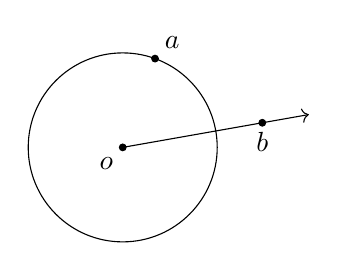
\begin{tikzpicture}[scale=0.6]
  \coordinate [label=below left:\(o\)]  (o) at (0  : 0);
  \draw [fill] (o) circle [radius=2pt];
  \coordinate [label=above right:\(a\)] (a) at (70 : 2);
  \draw [fill] (a) circle [radius=2pt];
  \coordinate [label=below:\(b\)]       (b) at (10 : 3);
  \draw [fill] (b) circle [radius=2pt];
  \draw [->] (o) -- (10: 4);
  \draw (o) circle [radius=2];
\end{tikzpicture}
\end{center}

\item[PG4.] \textbf{Interleaved Diameters.} Let \(C_1\) and \(C_2\) be circles centered at distinct points \(o_1\) and \(o_2\), respectively.
Further suppose we have diameters \(\SEGMENT{a_1}{b_1}\) of \(C_1\) and \(\SEGMENT{a_2}{b_2}\) of \(C_2\) such that \(\BETWEEN{a_1}{o_1}{a_2}\) and \(\BETWEEN{a_1}{o_2}{a_2}\).
Then \(C_1 \cap C_2\) is nonempty if and only if \(\BETWEENS{a_1b_2b_1a_2}\), and in this case \(C_1 \cap C_2\) consists of exactly two points which are on opposite sides of \(\LINE{o_1}{o_2}\).

\begin{center}
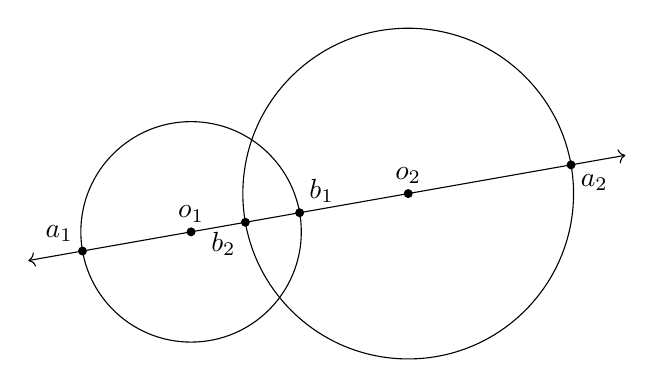
\begin{tikzpicture}[scale=0.7]
  \coordinate [label=above:{\(o_1\)}]  (o1) at (0,0);
  \draw [fill] (o1) circle [radius=2pt];
  \coordinate [label=above left:{\(a_1\)}] (a1) at ($ (o1)+(10 : -2) $);
  \draw [fill] (a1) circle [radius=2pt];
  \coordinate [label=above right:{\(b_1\)}] (b1) at ($ (o1)+(10 : 2) $);
  \draw [fill] (b1) circle [radius=2pt];
  \draw (o1) circle [radius=2];
  \coordinate [label=above:\(o_2\)]  (o2) at ($ (o1)+(10 : 4) $);
  \draw [fill] (o2) circle [radius=2pt];
  \coordinate [label=below right:\(a_2\)] (a2) at ($ (o2)+(10 : 3) $);
  \draw [fill] (a2) circle [radius=2pt];
  \coordinate [label=below left:\(b_2\)] (b2) at ($ (o2)+(10 : -3) $);
  \draw [fill] (b2) circle [radius=2pt];
  \draw (o2) circle [radius=3];
  \draw [<->] ($ (o1)+(10 : -3) $) -- ($ (o2)+(10 : 4) $);
\end{tikzpicture}
\end{center}
\end{proplist}
\end{dfn}

Each of these properties says something which is (hopefully!) fairly intuitive.
Angle-Side Congruence provides an essential link between segment congruence and angle congruence, which are otherwise unrelated.
The Circle Cut and Interleaved Diameters properties allow us to construct points on the intersection of a circle with a central ray and of two circles, respectively.
(Without these we have no way to construct points on circles!)

We finally have enough technology to start doing some more recognizable geometry.
For the remainder of this chapter \(P\) is a plane geometry.
First, we give two shortcut results for determining when two triangles are congruent.

\begin{prop}[SSS Theorem]\label{prop:sss-theorem}
If two nondegenerate triangles can be labeled such that corresponding sides are congruent, then the triangles are congruent.

More precisely, let \(a_1\), \(b_1\), and \(c_1\) be distinct points and \(a_2\), \(b_2\), and \(c_2\) be distinct points.
If \(\SEGMENT{a_1}{b_1} \equiv \SEGMENT{a_2}{b_2}\), \(\SEGMENT{b_1}{c_1} \equiv \SEGMENT{b_2}{c_2}\), and \(\SEGMENT{c_1}{a_1} \equiv \SEGMENT{c_2}{a_2}\), then \(\TRIANGLE{a_1}{b_1}{c_1} \equiv \TRIANGLE{a_2}{b_2}{c_2}\).
\end{prop}

\begin{proof}
We have \(\ANGLE{a_1}{b_1}{c_1} \equiv \ANGLE{a_2}{b_2}{c_2}\), \(\ANGLE{b_1}{c_1}{a_1} \equiv \ANGLE{b_2}{c_2}{a_2}\), and \(\ANGLE{c_1}{a_1}{b_1} \equiv \ANGLE{c_2}{a_2}{b_2}\) using the Angle-Side Congruence property three times.
\end{proof}

\begin{prop}[SAS Theorem]\label{prop:sas-theorem}
If two nondegenerate triangles can be labeled such that two corresponding sides, and the angles between, are congruent, then the triangles are congruent.

More precisely, let \(a_1\), \(b_1\), and \(c_1\) be distinct points, and \(a_2\), \(b_2\), and \(c_2\) be distinct points.
If \(\SEGMENT{a_1}{b_1} \equiv \SEGMENT{a_2}{b_2}\), \(\SEGMENT{b_1}{c_1} \equiv \SEGMENT{b_2}{c_2}\), and \(\ANGLE{a_1}{b_1}{c_1} \equiv \ANGLE{a_2}{b_2}{c_2}\), then \(\TRIANGLE{a_1}{b_1}{c_1} \equiv \TRIANGLE{a_2}{b_2}{c_2}\).
\end{prop}

\begin{proof}
We have \(\SEGMENT{a_1}{c_1} \equiv \SEGMENT{a_2}{c_2}\) by Angle-Side Congruence, and then \hyperref[prop:sss-theorem]{SSS} applies.
\end{proof}

\begin{cor}[Pons Asinorum]\label{cor:pons-asinorum}
If \(\TRIANGLE{a}{b}{c}\) is isoceles with \(\SEGMENT{a}{b} \equiv \SEGMENT{b}{c}\), then \(\ANGLE{b}{a}{c} \equiv \ANGLE{b}{c}{a}\).
\end{cor}

\begin{proof}
We have two triangles, \(\TRIANGLE{b}{a}{c}\) and \(\TRIANGLE{b}{c}{a}\), such that \(\SEGMENT{b}{c}\equiv \SEGMENT{b}{a}\), \(\SEGMENT{b}{a} \equiv \SEGMENT{b}{c}\), and \(\ANGLE{c}{b}{a} \equiv \SEGMENT{a}{b}{c}\).
By \hyperref[prop:sas-theorem]{SAS} we have \(\TRIANGLE{b}{a}{c} \equiv \TRIANGLE{b}{c}{a}\), and thus \(\ANGLE{b}{a}{c} \equiv \ANGLE{b}{c}{a}\) as needed.
\end{proof}

\begin{cor}
Every triangle which is equilateral is also equiangular; all three interior angles are congruent.
\end{cor}

\begin{proof}
Follows from two applications of Pons Asinorum.
\end{proof}

\begin{cor}[Segment Addition]\label{cor:segment-addition}
Suppose \(\BETWEEN{a_1}{b_1}{c_1}\) and \(\BETWEEN{a_2}{b_2}{c_2}\).
If any two of \(\SEGMENT{a_1}{b_1} \equiv \SEGMENT{a_2}{b_2}\), \(\SEGMENT{b_1}{c_1} \equiv \SEGMENT{b_2}{c_2}\), and \(\SEGMENT{a_1}{c_1} \equiv \SEGMENT{a_2}{c_2}\) hold, then so does the third.
\end{cor}

\begin{proof}
Note that \(\ANGLE{a_1}{b_1}{c_1} \equiv \ANGLE{a_2}{b_2}{c_2}\), \(\ANGLE{b_1}{c_1}{a_1} \equiv \ANGLE{b_2}{c_2}{a_2}\), and \(\ANGLE{c_1}{a_1}{b_1} \equiv \ANGLE{c_2}{a_2}{b_2}\) by AC1.
The result then follows from three applications of \hyperref[prop:sas-theorem]{SAS}.
\end{proof}

\begin{dfn}[Antipode]
Let \(a\), \(b\), and \(c\) be points.
We say that \(c\) is an \emph{antipode}\index{antipode} of \(a\) \emph{through} \(b\) if \(\BETWEEN{a}{b}{c}\) and \(\SEGMENT{a}{b} \equiv \SEGMENT{b}{c}\).
\end{dfn}

\begin{construct}[Antipode]\label{construct:antipode}
Given distinct points \(a\) and \(b\), there is a unique point \(c\) such that \(c\) is an antipode of \(a\) through \(b\).
\end{construct}

\begin{proof}
First we show existence.
Using the Interpolation property, there is a point \(u\) such that \(\BETWEEN{u}{b}{a}\).
Now using Circle Cut, there is a point \(c \in \RAY{b}{u} \cap \CIRCLE{b}{a}\).
Note that \(\BETWEEN{a}{b}{c}\), and we have \(\SEGMENT{b}{c} \equiv \SEGMENT{b}{a}\) as needed.
Next we show uniqueness.
Suppose \(d\) is a point such that \(\BETWEEN{a}{b}{d}\) and \(\SEGMENT{a}{b} \equiv \SEGMENT{b}{d}\).
But then \(d \in \RAY{b}{c}\), and in fact \(c = d\) by AC4.
\end{proof}

\begin{construct}[Equilateral triangle with a given side]\label{construct:equilateral-points}
Given distinct points \(a\) and \(b\), there exist points \(c_1\) and \(c_2\), on opposite sides of \(\LINE{a}{b}\), such that \(\TRIANGLE{a}{b}{c_1}\) and \(\TRIANGLE{a}{b}{c_2}\) are equilateral.
In fact, we have \(\TRIANGLE{a}{b}{c_1} \equiv \TRIANGLE{a}{b}{c_2}\).
\end{construct}

\begin{proof}
First, construct the antipode \(h\) of \(b\) through \(a\), and construct the antipode \(k\) of \(a\) through \(b\).
Note that \(\BETWEENS{habk}\), and that \(\SEGMENT{a}{h} \equiv \SEGMENT{a}{b}\) and \(\SEGMENT{b}{k} \equiv \SEGMENT{b}{a}\); that is, \(a\) is a midpoint of \(\SEGMENT{h}{b}\) and \(b\) a midpoint of \(\SEGMENT{a}{k}\), so that \(a\) is the center of \(\CIRCLE{a}{b}\) with diameter \(\SEGMENT{h}{b}\) and \(b\) is the center of \(\CIRCLE{b}{a}\) with diameter \(\SEGMENT{a}{k}\).
Thus the Interleaved Diameters property applies, and we have two points \(c_1,c_2 \in \CIRCLE{a}{b} \cap \CIRCLE{b}{a}\) which are in opposite halfplanes of \(\LINE{a}{b}\).
Note that \(\SEGMENT{a}{c_1} \equiv \SEGMENT{a}{b} \equiv \SEGMENT{b}{c_1}\), and thus \(\TRIANGLE{a}{b}{c_1}\) is equilateral.
Similarly, \(\TRIANGLE{a}{b}{c_2}\) is equilateral.
Moreover, we see that \(\TRIANGLE{a}{b}{c_1} \equiv \TRIANGLE{a}{b}{c_2}\) by the SSS Theorem.
\end{proof}

\begin{lem}[Betweenness Transfer]\label{lem:betweenness-transfer}
Suppose \(\BETWEEN{a}{b}{c}\) and \(y \in \RAY{x}{z}\).
If \(\SEGMENT{a}{b} \equiv \SEGMENT{x}{y}\) and \(\SEGMENT{a}{c} \equiv \SEGMENT{x}{z}\), then \(\BETWEEN{x}{y}{z}\).
\end{lem}

\begin{proof}
Since \(y \in \RAY{x}{z}\), we have four possibilities: \(y = x\), \(\BETWEEN{x}{y}{z}\), \(y = z\), and \(\BETWEEN{x}{z}{y}\).
If \(y = x\), then we have \(\SEGMENT{a}{b} \equiv \SEGMENT{x}{x}\), so that \(b = a\), a contradiction.
Similarly if \(y = z\) then we have \(\SEGMENT{a}{b} \equiv \SEGMENT{x}{y} \equiv \SEGMENT{x}{z} \equiv \SEGMENT{a}{c}\), so that \(b = c\), also a contradiction.
Now suppose that \(\BETWEEN{x}{z}{y}\).
Note that \(\ANGLE{c}{a}{b} \equiv \ANGLE{z}{x}{y}\), \(\SEGMENT{a}{c} \equiv \SEGMENT{x}{z}\), and \(\SEGMENT{a}{b} \equiv \SEGMENT{x}{y}\); by \hyperref[prop:sas-theorem]{SAS}, \(\TRIANGLE{a}{b}{c} \equiv \TRIANGLE{x}{y}{z}\).
In particular, the flat angle \(\ANGLE{a}{c}{b}\) is congruent to the straight angle \(\ANGLE{x}{z}{y}\), a contradiction.
Thus \(\BETWEEN{x}{y}{z}\) as claimed.
\end{proof}

\begin{construct}[Segment Copy Theorem]
Let \(a\) and \(b\) be distinct points, and let \(o\) and \(t\) be distinct points.
Then there is a unique point \(x\) on \(\RAY{o}{t}\) such that \(\SEGMENT{o}{x} \equiv \SEGMENT{a}{b}\).
\end{construct}

\begin{proof}
First we construct a point \(z\) such that \(\TRIANGLE{a}{o}{z}\) is equilateral; now \(\SEGMENT{z}{a} \equiv \SEGMENT{z}{o}\).
Using the Interpolation property, construct a point \(h\) such that \(\BETWEEN{z}{a}{h}\), and using the Circle Cut property, construct a point \(u\) on \(\RAY{a}{h}\) such that \(\SEGMENT{a}{u} \equiv \SEGMENT{a}{b}\).
Again using Circle Cut, construct a point \(v\) on \(\RAY{z}{o}\) such that \(\SEGMENT{z}{v} \equiv \SEGMENT{z}{u}\).
By \lemref{lem:betweenness-transfer} we have \(\BETWEEN{z}{o}{v}\).
Now \(\SEGMENT{z}{a} \equiv \SEGMENT{z}{o}\) and \(\SEGMENT{z}{u} \equiv \SEGMENT{z}{v}\), thus \(\SEGMENT{a}{u} \equiv \SEGMENT{o}{v}\).
Again using Circle Cut, construct a point \(x\) on \(\RAY{o}{t}\) such that \(\SEGMENT{o}{x} \equiv \SEGMENT{o}{v}\).
Then we have \(\SEGMENT{o}{x} \equiv \SEGMENT{o}{v} \equiv \SEGMENT{a}{u} \equiv \SEGMENT{a}{b}\) as needed.
Uniqueness follows from SC3.
\end{proof}

\begin{construct}[Angle Copy Theorem]
Let \(a\), \(o\), \(b\) be distinct noncollinear points and let \(P\) and \(x\) be distinct points.
There exist two points \(y_1\) and \(y_2\), on opposite sides of \(\LINE{p}{x}\), such that \(\ANGLE{x}{p}{y_1} \equiv \ANGLE{x}{p}{y_2} \equiv \ANGLE{a}{o}{b}\). 
\end{construct}

\begin{proof}
First copy segment \(\SEGMENT{o}{b}\) onto \(\RAY{p}{x}\) at the point \(u\), then copy the segment \(\SEGMENT{b}{a}\) onto the ray \(\RAY{u}{p}\) at the point \(v\).
Now copy \(\SEGMENT{o}{a}\) onto \(\RAY{p}{x}\) at the point \(w\).
Note that \(\SEGMENT{o}{a} \equiv \SEGMENT{p}{w}\), \(\SEGMENT{o}{b} \equiv \SEGMENT{p}{u}\), and \(\SEGMENT{b}{a} \equiv \SEGMENT{u}{v}\).
Moreover, the intersection \(\CIRCLE{o}{a} \cap \CIRCLE{b}{a}\) is nonempty, as it contains \(a\).
By the Interleaved Diameters property, \(\CIRCLE{p}{w} \cap \CIRCLE{u}{v}\) contains two points \(z_1\) and \(z_2\) on opposite sides of \(\LINE{p}{x}\).
By the SSS Theorem, we have \(\TRIANGLE{p}{u}{z_1} \equiv \TRIANGLE{o}{b}{a} \equiv \TRIANGLE{p}{u}{z_2}\), and thus \(\ANGLE{u}{p}{z_1} \equiv \ANGLE{a}{o}{b} \equiv \ANGLE{u}{p}{z_2}\) as needed.
\end{proof}

\begin{prop}[ASA Theorem]
Let \(a\), \(b\), \(c\) be distinct noncollinear points, and let \(x\), \(y\), \(z\) be distinct points.
If \(\ANGLE{a}{b}{c} \equiv \ANGLE{x}{y}{z}\), \(\SEGMENT{b}{c} \equiv \SEGMENT{y}{z}\), and \(\ANGLE{b}{c}{a} \equiv \ANGLE{y}{z}{x}\), then \(\TRIANGLE{a}{b}{c} \equiv \TRIANGLE{x}{y}{z}\).
\end{prop}

\begin{proof}
Copy \(\SEGMENT{y}{x}\) onto \(\RAY{b}{a}\) at \(d\).
Note that \(d\) and \(a\) are on the same side of \(\LINE{b}{c}\).
Moreover, we have \(\TRIANGLE{d}{b}{c} \equiv \TRIANGLE{x}{y}{z}\) by the SAS Theorem, and so \(\ANGLE{b}{c}{d} \equiv \ANGLE{y}{z}{x} \equiv \ANGLE{b}{c}{a}\).
By AC4, we have \(d \in \RAY{c}{a}\).
Now \(d\) is on both \(\LINE{b}{a}\) and \(\LINE{c}{a}\), and since \(a\), \(b\), and \(c\) are not collinear, we must have \(d = a\).
So \(\TRIANGLE{a}{b}{c} \equiv \TRIANGLE{x}{y}{z}\) as claimed.
\end{proof}

    \newpage

  \section{Transversals}
    \begin{prop}[Supplements are unique] \mbox{}
\begin{proplist}
\item Suppose that \(\ANGLE{a_1}{o_1}{b_1}\) and \(\ANGLE{b_1}{o_1}{c_1}\) are a linear pair, and that \(\ANGLE{a_2}{o_2}{b_2}\) and \(\ANGLE{b_2}{o_2}{c_2}\) are a linear pair.
If \(\ANGLE{a_1}{o_1}{b_1} \equiv \ANGLE{a_2}{o_2}{b_2}\), then \(\ANGLE{b_1}{o_1}{c_1} \equiv \ANGLE{b_2}{o_2}{c_2}\).

\begin{center}
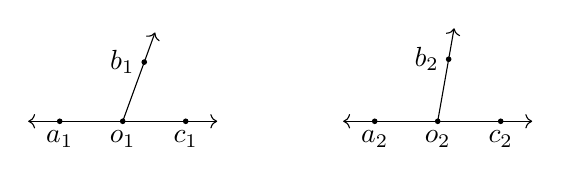
\begin{tikzpicture}[scale=0.8]
  \coordinate [label=below:\(o_1\)] (o1) at (-3,0);
  \coordinate [label=below:\(a_1\)] (a1) at ($ (o1)+(180:1) $);
  \coordinate [label=left:\(b_1\)] (b1) at ($ (o1)+(70:1) $);
  \coordinate [label=below:\(c_1\)] (c1) at ($ (o1)+(0:1) $);

  \draw [fill] (o1) circle [radius=1pt];
  \draw [fill] (a1) circle [radius=1pt];
  \draw [fill] (b1) circle [radius=1pt];
  \draw [fill] (c1) circle [radius=1pt];

  \draw [->] (o1) -- ($ (a1)+(180:0.5) $);
  \draw [->] (o1) -- ($ (b1)+(70:0.5) $);
  \draw [->] (o1) -- ($ (c1)+(0:0.5) $);

  \coordinate [label=below:\(o_2\)] (o2) at (2,0);
  \coordinate [label=below:\(a_2\)] (a2) at ($ (o2)+(180:1) $);
  \coordinate [label=left:\(b_2\)] (b2) at ($ (o2)+(80:1) $);
  \coordinate [label=below:\(c_2\)] (c2) at ($ (o2)+(0:1) $);

  \draw [fill] (o2) circle [radius=1pt];
  \draw [fill] (a2) circle [radius=1pt];
  \draw [fill] (b2) circle [radius=1pt];
  \draw [fill] (c2) circle [radius=1pt];

  \draw [->] (o2) -- ($ (a2)+(180:0.5) $);
  \draw [->] (o2) -- ($ (b2)+(80:0.5) $);
  \draw [->] (o2) -- ($ (c2)+(0:0.5) $);
\end{tikzpicture}
\end{center}

\item Suppose \(\alpha\), \(\beta\), and \(\gamma\) are angles such that \(\alpha\) and \(\beta\) are supplementary and \(\alpha\) and \(\gamma\) are supplementary.
Then \(\alpha \equiv \gamma\).
\end{proplist}
\end{prop}

\begin{proof}\mbox{}
\begin{proplist}
\item Suppose we have two such linear pairs.
Without loss of generality, we can suppose that \[ \SEGMENT{o_1}{a_1} \equiv \SEGMENT{o_1}{b_1} \equiv \SEGMENT{o_1}{c_1} \equiv \SEGMENT{o_2}{a_2} \equiv \SEGMENT{o_2}{b_2} \equiv \SEGMENT{o_2}{c_2}. \] (If they aren't, we can use Circle Cut and the Segment Copy construction to find such points.) Now \(\TRIANGLE{b_1}{o_1}{a_1} \equiv \TRIANGLE{b_2}{o_2}{a_2}\) by SAS, so that \(\ANGLE{b_1}{a_1}{o_1} \equiv \ANGLE{b_2}{a_2}{o_2}\).
Now \(\SEGMENT{a_1}{c_1} \equiv \SEGMENT{a_2}{c_2}\), so that \(\TRIANGLE{b_1}{a_1}{c_1} \equiv \TRIANGLE{b_2}{a_2}{c_2}\) by SAS.
So \(\SEGMENT{b_1}{c_1} \equiv \SEGMENT{b_2}{c_2}\), and thus \(\TRIANGLE{b_1}{o_1}{c_1} \equiv \TRIANGLE{b_2}{o_2}{c_2}\) by SSS.
Thus \(\ANGLE{b_1}{o_1}{c_1} \equiv \ANGLE{b_2}{o_2}{c_2}\) as needed.

\item Follows from the definition of supplementary.
\qedhere
\end{proplist}
\end{proof}

\begin{cor}
If angles \(\alpha\) and \(\beta\) are a vertical pair, then \(\alpha \equiv \beta\).
\end{cor}

\begin{proof}
If \(\ANGLE{a}{o}{b}\) and \(\ANGLE{c}{o}{d}\) are a vertical pair, with \(\BETWEEN{b}{o}{c}\) and \(\BETWEEN{a}{o}{d}\), then both \(\ANGLE{a}{o}{b}\) and \(\ANGLE{c}{o}{d}\) are supplementary to \(\ANGLE{a}{o}{c}\).
\end{proof}


\begin{dfn}[Transversal]
Suppose we have three lines \(\ell_1\), \(\ell_2\), and \(t\) in a plane geometry.
We say that \(t\) is a \emph{transversal}\index{transversal} of \(\ell_1\) and \(\ell_2\) if \(t\) cuts both \(\ell_1\) and \(\ell_2\) at unique points, and these points are distinct.

Suppose \(t\) is a transversal of \(\ell_1\) and \(\ell_2\), cutting these lines at \(o_1\) and \(o_2\), respectively as shown.

\begin{center}
\begin{tikzpicture}[scale=0.5]
  \coordinate (x1) at (-5,0);
  \coordinate (y1) at (4,0);
  \draw [<->] (x1) -- (y1);
  \node at (4,-0.5) {\(\ell_1\)};
  \coordinate (x2) at (-4,5);
  \coordinate (y2) at (4,3);
  \draw [<->] (x2) -- (y2);
  \node  at (-3,5.5) {\(\ell_2\)};
  \coordinate (x3) at (-1,-1);
  \coordinate (y3) at (1,6);
  \draw [<->] (x3) -- (y3);
  \node at (0.7,6) {\(t\)};
  \coordinate [label=below right:\(o_1\)] (o1) at (intersection of x1--y1 and x3--y3);
  \draw [fill] (o1) circle [radius=1pt];
  \coordinate [label=below left:\(o_2\)] (o2) at (intersection of x2--y2 and x3--y3);
  \draw [fill] (o2) circle [radius=1pt];
  \coordinate (x4) at (-0.5,2);
  \coordinate (y4) at (1,3);
  \coordinate [label=below:\(a\)] (a) at (intersection of x1--y1 and x4--y4);
  \draw [fill] (a) circle [radius=1pt];
  \coordinate [label=below:\(b\)] (b) at (intersection of x2--y2 and x4--y4);
  \draw [fill] (b) circle [radius=1pt];
\end{tikzpicture}
\end{center}

If \(a\) is on \(\ell_1\) and \(b\) is on \(\ell_2\) such that \(a\) and \(b\) are on opposite sides of \(t\), then we say that \(\ANGLE{a}{o_1}{o_2}\) and \(\ANGLE{b}{o_2}{o_1}\) are \emph{alternate interior angles}\index{alternate interior angles} of this transversal.
\end{dfn}

Every transversal has two pairs of alternate interior angles.

\begin{prop}[Alternate Interior Angles]\label{prop:aia-theorem}
If two lines \(\ell_1\) and \(\ell_2\) are cut by a transversal \(t\) so that a pair of alternate interior angles are congruent, then \(\ell_1\) and \(\ell_2\) are parallel.
\end{prop}

\begin{proof}
Suppose \(t\) meets \(\ell_1\) and \(\ell_2\) at points \(o_1\) and \(o_2\) respectively, and that \(a\) and \(b\) are on \(\ell_1\) and \(\ell_2\), respectively, and on opposite sides of \(t\), such that \(\ANGLE{a}{o_1}{o_2} \equiv \ANGLE{b}{o_2}{o_1}\).
Now suppose by way of contradiction that \(\ell_1\) and \(\ell_2\) are \emph{not} parallel; rather, they meet at a point \(x\) which (WLOG) is on the \(a\)-side of \(t\).
Let \(c\) be on \(\ell_1\) such that \(\BETWEEN{a}{o_1}{c}\).
Copy \(\SEGMENT{o_1}{x}\) onto \(\RAY{o_2}{b}\) at the point \(y\).
Note that \(\SEGMENT{o_1}{x} \equiv \SEGMENT{o_2}{y}\), \(\SEGMENT{o_1}{o_2} \equiv \SEGMENT{o_2}{o_1}\), and \(\ANGLE{x}{o_1}{o_2} \equiv \ANGLE{y}{o_2}{o_1}\); by \hyperref[prop:sas-theorem]{SAS} we thus have \(\TRIANGLE{x}{o_1}{o_2} \equiv \TRIANGLE{y}{o_2}{o_1}\).
In particular, \(\ANGLE{o_2}{o_1}{y} \equiv \ANGLE{o_1}{o_2}{x}\).

\begin{center}
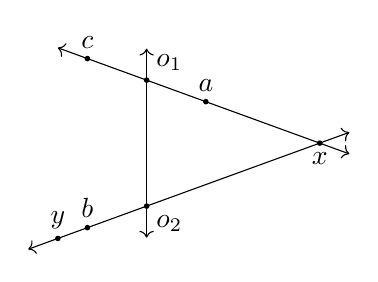
\begin{tikzpicture}[scale=0.8]
  \coordinate [label=above right:\(o_1\)] (o1) at (0,2);
  \coordinate [label=below right:\(o_2\)] (o2) at ($ (o1)+(270:2) $);
  \coordinate [label=above:\(a\)] (a) at ($ (o1)+(160:-1) $);
  \coordinate [label=above:\(c\)] (c) at ($ (o1)+(160:1) $);
  \coordinate [label=above:\(b\)] (b) at ($ (o2)+(200:1) $);
  \coordinate [label=below:\(x\)] (x) at (intersection of o1--a and o2--b);
  \coordinate [label=above:\(y\)] (y) at ($ (o2)+(200:1.5) $);

  \draw [fill] (o1) circle [radius=1pt];
  \draw [fill] (o2) circle [radius=1pt];
  \draw [fill] (a) circle [radius=1pt];
  \draw [fill] (c) circle [radius=1pt];
  \draw [fill] (b) circle [radius=1pt];
  \draw [fill] (x) circle [radius=1pt];
  \draw [fill] (y) circle [radius=1pt];

  \draw [<->] ($ (o1)+(90:0.5) $) -- ($ (o2)+(270:0.5) $);
  \draw [<->] ($ (y)+(200:0.5) $) -- ($ (x)+(200:-0.5) $);
  \draw [<->] ($ (c)+(160:0.5) $) -- ($ (x)+(160:-0.5) $);
\end{tikzpicture}
\end{center}

Note that \(\ANGLE{x}{o_2}{o_1}\) and \(\ANGLE{o_1}{o_2}{y}\) are supplementary, and \(\ANGLE{o_1}{o_2}{y} \equiv \ANGLE{a}{o_1}{o_2}\) by hypothesis, so that \(\ANGLE{a}{o_1}{o_2}\) and \(\ANGLE{x}{o_2}{o_1}\) are supplementary.
Since \(\ANGLE{x}{o_2}{o_1} \equiv \ANGLE{y}{o_1}{o_2}\), we have that \(\ANGLE{a}{o_1}{o_2}\) and \(\ANGLE{y}{o_1}{o_2}\) are supplementary.
But also \(\ANGLE{a}{o_1}{o_2}\) and \(\ANGLE{o_2}{o_1}{c}\) are supplementary.
Thus \(\ANGLE{o_2}{o_1}{y} \equiv \ANGLE{o_2}{o_1}{c}\).
By AC4, we have that \(o_1\), \(c\), and \(y\) are collinear, so that \(y \in \ell_1\).
But now \(\ell_1\) and \(\ell_2\) have two points in common -- \(x\) and \(y\) -- which are necessarily distinct as they are on opposite halfplanes of \(t\).
So we have \(\ell_1 = \ell_2\), a contradiction.

Thus \(\ell_1\) and \(\ell_2\) must be parallel. 
\end{proof}

\begin{prop}[AAS Theorem]\label{prop:aas-theorem}
Suppose we have triangles \(\TRIANGLE{A}{B}{C}\) and \(\TRIANGLE{X}{Y}{Z}\) such that \(\ANGLE{C}{A}{B} \equiv \ANGLE{Z}{X}{Y}\), \(\ANGLE{A}{B}{C} \equiv \ANGLE{X}{Y}{Z}\), and \(\SEGMENT{B}{C} \equiv \SEGMENT{Y}{Z}\).
Then \(\TRIANGLE{A}{B}{C} \equiv \TRIANGLE{X}{Y}{Z}\).
\end{prop}

\begin{proof}
Copy \(\SEGMENT{B}{A}\) onto \(\RAY{Y}{X}\) at the point \(W\).
Note that \(\TRIANGLE{W}{Y}{Z} \equiv \TRIANGLE{A}{B}{C}\) by SAS, so that \(\ANGLE{B}{A}{C} \equiv \TRIANGLE{Y}{W}{Z}\).
Suppose now that \(W\) and \(X\) are distinct points.
In this case \(\LINE{X}{Z}\) and \(\LINE{W}{Z}\) are lines cut by a transversal \(\LINE{X}{Y}\).
Moreover, if we let \(U\) be a point such that \(\BETWEEN{U}{X}{Z}\), then \(\ANGLE{U}{X}{W}\) and \(\ANGLE{Y}{X}{Z}\) are vertical, hence congruent, and so \(\ANGLE{U}{X}{W} \equiv \ANGLE{Y}{X}{Z}\).
But now by the Alternate Interior Angles theorem \(\LINE{X}{Z}\) and \(\LINE{W}{Z}\) must be parallel, a contradiction since they meet at \(Z\).
So in fact \(X\) and \(W\) are the same point, and thus \(\TRIANGLE{A}{B}{C} \equiv \TRIANGLE{X}{Y}{Z}\) by SAS.
\end{proof}

\begin{prop}[HL Theorem]
Let \(\TRIANGLE{A}{B}{C}\) and \(\TRIANGLE{X}{Y}{Z}\) be triangles such that \(\ANGLE{B}{C}{A}\) and \(\ANGLE{Y}{Z}{X}\) are right and \(\SEGMENT{A}{B} \equiv \SEGMENT{X}{Y}\) and \(\SEGMENT{B}{C} \equiv \SEGMENT{Y}{Z}\).
Then \(\TRIANGLE{A}{B}{C} \equiv \TRIANGLE{X}{Y}{Z}\).
\end{prop}

\begin{proof}
Copy \(\SEGMENT{Z}{X}\) onto the ray opposite \(\RAY{C}{A}\) at the point \(D\).
Now \(\ANGLE{B}{C}{D}\) is a right angle, since it is supplementary to \(\ANGLE{A}{C}{B}\).
By SAS, we have \(\TRIANGLE{X}{Y}{Z} \equiv \TRIANGLE{D}{C}{B}\), and thus \(\SEGMENT{B}{D} \equiv \SEGMENT{Y}{X} \equiv \SEGMENT{B}{A}\).
Now \(\TRIANGLE{A}{B}{D}\) is isoceles with \(\SEGMENT{B}{A} \equiv \SEGMENT{B}{D}\), so that \(\ANGLE{B}{A}{C} \equiv \ANGLE{B}{A}{D} \equiv \ANGLE{B}{D}{A} \equiv \ANGLE{Y}{X}{Z}\).
By AAS, we have \(\TRIANGLE{A}{B}{C} \equiv \TRIANGLE{X}{Y}{Z}\).
\end{proof}

\begin{prop}
A triangle formed by three noncollinear points cannot have two interior angles which are both right.
\end{prop}

\begin{proof}
Such a triangle would violate the Alternate Interior Angles theorem since right angles are self-supplementary, and any two right angles are congruent.
\end{proof}


\begin{construct}[Angle Bisector]
Let \(A\), \(O\), and \(B\) be noncollinear points.
There exists a unique line \(\ell\), containing \(O\), such that if \(U \in \ell\) is different from \(O\) then \(\ANGLE{A}{O}{U} \equiv \ANGLE{B}{O}{U}\).
This line is called the \emph{bisector} of \(\ANGLE{A}{O}{B}\).
\end{construct}

\begin{proof}
Note that we can assume WLOG that \(\SEGMENT{O}{A} \equiv \SEGMENT{O}{B}\); if not, construct such a point on \(\RAY{O}{B}\) using the Circle Separation property.
Since the intersection of \(\CIRCLE{A}{O}\) and \(\CIRCLE{B}{O}\) contains a point not on \(\LINE{A}{B}\), by Circle Cut Transfer there is a second point \(U\) on the opposite side of \(\LINE{A}{B}\) such that \(\SEGMENT{A}{U} \equiv \SEGMENT{B}{U}\).
Let \(\ell = \LINE{O}{U}\).
Note that \(\TRIANGLE{A}{O}{U} \equiv \TRIANGLE{B}{O}{U}\) by SSS, so that \(\ANGLE{A}{O}{U} \equiv \ANGLE{B}{O}{U}\).
Then if \(V\) is a point such that \(\BETWEEN{V}{O}{U}\), we have \(\ANGLE{V}{O}{A} \equiv \ANGLE{V}{O}{B}\), since these are supplementary to congruent angles.

To see uniqueness, note that any such line must contain \(O\) and \(U\).
\end{proof}

\begin{cor}
\(A\) and \(B\) are on opposite sides of the bisector of \(\ANGLE{A}{O}{B}\).
In particular, the bisector of \(\ANGLE{A}{O}{B}\) contains points which are interior to \(\ANGLE{A}{O}{B}\).
\end{cor}

\begin{proof}
Suppose otherwise, and let \(U \neq O\) be a point on the bisector.
Then \(\ANGLE{U}{O}{A}\) and \(\ANGLE{U}{O}{B}\) are congruent angles on the same half-plane of a ray, so that \(A\), \(B\), and \(O\) are collinear -- a contradiction.
By the plane separation property there is a point \(W\) between \(A\) and \(B\) which is on the bisector; this point is interior to \(\ANGLE{A}{O}{B}\) as needed.
\end{proof}

\begin{construct}[Segment Midpoint]
Let \(A\) and \(B\) be distinct points.
There is a unique point \(M\) such that \(\BETWEEN{A}{M}{B}\) and \(\SEGMENT{A}{M} \equiv \SEGMENT{B}{M}\).
This point is called the \emph{midpoint} of \(\SEGMENT{A}{B}\).
\end{construct}

\begin{proof}
Construct a point \(O\) such that \(\TRIANGLE{A}{O}{B}\) is equilateral, and construct the bisector of \(\ANGLE{A}{O}{B}\).
By the Crossbar theorem, this bisector must cut \(\SEGMENT{A}{B}\) at an interior point, say \(M\).
Now \(\TRIANGLE{O}{A}{M} \equiv \TRIANGLE{O}{B}{M}\) by SAS, and thus \(\SEGMENT{A}{M} \equiv \SEGMENT{B}{M}\) as needed.
Note that \(M\) is unique by the uniqueness of congruent segments on a ray.
\end{proof}

    \newpage

  \section{Perpendiculars and Tangents}
    \input{src/geo/4.03-perpendiculars-and-tangents.tex}
    \newpage

  \section{Incircles and Excircles}
    \input{src/geo/4.04-incircles-and-excircles.tex}


\chapter{Models}
\newpage

  \section{\(\RR^2\) -- The Cartesian Plane}
    \input{src/geo/5.01-cartesian-plane-model.tex}
    \newpage

  \section{\(\HYPHP\) -- The Hyperbolic Half Plane}
    \input{src/geo/5.02-hyperbolic-half-plane-model.tex}
    \newpage

  \section{\(\POINCAREDISC\) -- The Poincare Disc}
    \input{src/geo/5.03-poincare-disc-model.tex}
    \newpage

  \section{\(\KLEINDISC\) -- The Klein Disc}
    \input{src/geo/5.04-klein-disc-model.tex}
    \newpage

  \section{\(\GANSDISC\) -- The Gans Disc}
    \input{src/geo/5.05-gans-disc-model.tex}


\backmatter
  \bibliographystyle{plain}
  \bibliography{src/bibliography}

  \printindex

\end{document}
